\section{Advanced analysis}
Suppose that national government apply a national lockdown to contain inferction, when they exceed a threshold $\delta$.

In following section will be added a new assumption for model \ref{eq:sir_model}:

\begin{itemize}
    \item Lockdown has been modelled as a rate infection $\beta = 0$.
\end{itemize}

System \ref{eq:sir_model_3} can be rimodelled as a Filippov system

\begin{equation}
    \label{eq:sir_model_pws_1}
    \begin{pmatrix} \dot{x_s} \\ \dot{x_i} \end{pmatrix} =
    \begin{cases}
        f^- =
        \begin{pmatrix} \mu - \beta x_sx_i - \mu x_s \\ \beta x_sx_i - (\gamma + \mu)x_i \end{pmatrix}
        & if\;H(x) < 0 \\
        f^+ =
        \begin{pmatrix} \mu - \mu x_s \\ - (\gamma + \mu)x_i \end{pmatrix}
        & if\;H(x) > 0 \\
    \end{cases}
\end{equation}

Where $H(x) = x_i - \delta$.

Notice that at discontinuity surface

\begin{equation}
    f^- = \begin{pmatrix} \mu - \left(\beta\delta + \mu\right) x_s \\ \beta\delta x_s - (\gamma + \mu)\delta \end{pmatrix} \neq \begin{pmatrix} \mu - \mu x_s \\ - (\gamma + \mu)\delta \end{pmatrix} = f^+
\end{equation}

So System (\ref{eq:sir_model_pws_1}) has a Degree of Discontiuity equal to 1 (Filippov System).

\subsection{Analysis of discontinuity surface}
Given that region of interest is Equation (\ref{eq:roi}), discontinuity surface can be restricred to

\begin{equation}
    \label{eq:switching_manifold}
    \Sigma = \{ (x_s,x_i) \in \mathbb{R}^2 : x_i = 1-\delta, 0 \leq x_s \leq \delta \}
\end{equation}

Can be usefull understand when $\Sigma$ is a sliding surface or a crossing surface.

First of all, it needs to calculates following properties of vector field

\begin{equation}
    \nabla H = \left(\frac{\partial H}{\partial x_s}, \frac{\partial H}{\partial x_i}\right) = (0,1)
\end{equation}

\begin{equation}
    \label{eq:f-}
    f^-_N = \nabla H f^- = \beta x_sx_i-(\gamma + \mu)x_i
\end{equation}

\begin{equation}
    \label{eq:f+}
    f^+_N = \nabla H f^+ = -(\gamma + \mu)x_i
\end{equation}

\begin{lemma}
Given the system \ref{eq:sir_model_pws_1}, the surface $\Sigma$ is a crossing surface for $0 \leq x_s < \frac{1}{R_0}$.
\end{lemma}

\begin{proof}
By definition $\Sigma$ is a crossing region if $f^+_Nf^-_N > 0$. Ma

\begin{equation}
    f^+_Nf^-_N = \delta^2(\gamma + \mu)^2(1- R_0x_s)
\end{equation}

By assumption
\begin{itemize}
    \item $\delta > 0$
    \item $\gamma + \mu > 0$
\end{itemize}

So

\begin{equation}
    x_s < \frac{1}{R_0} \implies f^+_Nf^-_N > 0
\end{equation}

Moreove, since $0 \leq x_s$, ii happnes that $\Sigma$ is a crossing region for $0 \leq x_s < \frac{1}{R_0}$
\end{proof}

\begin{lemma}
Given System (\ref{eq:sir_model_pws_1}), region $\Sigma$ is an attractive surface for $\frac{1}{R_0} < x_s \leq 1$.
\end{lemma}

\begin{proof}
By definition, $\Sigma$ is an attractive surface if $f^+_N < 0$ and $f^-_N > 0$.

From Equation (\ref{eq:f+}), solving equation and remembering that $x_i = \delta$, it happens that

\begin{equation}
    f^+_N = -(\gamma + \mu)\delta
\end{equation}

By assumption:
\begin{itemize}
    \item $\delta > 0$
    \item $\gamma + \mu > 0$
\end{itemize}
So $f^+_N < 0 \;\;\;\;\; \forall x_s \in \Omega$

From Equation (\ref{eq:f-}), solving equation and remembering that $x_i = \delta$, it happens that

\begin{equation}
    f^-_N = \delta\beta\left(x_s-\frac{1}{R_0}\right)
\end{equation}

By assumption:
\begin{itemize}
    \item $\delta > 0$
    \item $\beta > 0$
\end{itemize}
So $\frac{1}{R_0} < x_s \leq 1 \implies f^-_N > 0$

As consequence $\Sigma$ is an attraction surface for $\frac{1}{R_0} < x_s \leq 1$ 
\end{proof}

Given previous Lemma, following Theorem is verified

\begin{theorem}
Given System (\ref{eq:sir_model_pws_1}), following statements are verified:
\begin{itemize}
    \item If $R_0 < 1$ the discontinuity surface $\Sigma$ is a crossing surface $\forall x_s \in \Sigma$;
    \item If $R_0 > 1$ the discontinuity surface $\Sigma$ is a crossing surface for $x_s < \frac{1}{R_0}$ and a sliding surface for $x_s > \frac{1}{R_0}$.
\end{itemize}
\end{theorem}

Given that there is a switching surface, will be usefull calculate vector field along it.

Applying Filippov convntion, vector field along sliding surface is

\begin{equation}
    \label{eq:switching_surface_vector_field_1}
    f_\Sigma = \alpha f^+ + (1-\alpha)f^-
\end{equation}

Choosing

\begin{equation}
    \label{eq:switching_surface_alpha}
    \alpha = \frac{f^-_N}{f^-_N-f^+_N} = \frac{R_0x_s-1}{R_0x_s}
\end{equation}

and substituiting Equation (\ref{eq:switching_surface_alpha}) in Equation (\ref{eq:switching_surface_vector_field_1}), remebering that along $\Sigma$ happens $x_i = \delta$,  it became

\begin{equation}
    \label{eq:switching_surface_vector_field_2}
    f_\Sigma = \begin{pmatrix} \mu - \mu x_s - (\gamma +\mu) \delta \\ 0 \end{pmatrix}
\end{equation}

\subsection{Calcolo dei punti di equilibrio}

First of calculate equilibria, will be useful enunciate some Lemma.

\begin{lemma}
\label{th:equilibria_lockdown}
The vector field $f^+$ defined in \ref{eq:sir_model_pws_1} has no one ammissible equilibrium point.
\end{lemma}

\begin{proof}
A point is a equilibrium point if vector field is null in that point. So

\begin{equation}
\label{eq:sir_lockdown_nullclines}
    \begin{array}{ccc}
        \mu - \mu x_s &=& 0  \\
        - (\gamma + \mu)x_i &=& 0 
    \end{array}
\end{equation}

From Equation (\ref{eq:sir_lockdown_nullclines}) we get

\begin{equation}
\label{eq:sir_lockdown_nullclines_demonstation}
    \begin{array}{ccc}
        x_s &=& 1  \\
        x_i &=& 0 
    \end{array}
\end{equation}

To get an ammisible equilibrium point, it must fulfill condition $H(x) > 0 \implies x_i > \delta$.
But for hypothesis $\delta > 0 = x_i$, so equilibrium point of $f^+$ is not ammissible.
\end{proof}

\begin{lemma}
\label{th:sliding_equilibria}
Sliding surface \ref{eq:switching_surface_vector_field_2} has an admissible equilibrium point at $x^*=(1-\delta\frac{\left(\gamma+\mu\right)}{\mu},\delta)$ if and only if $R_0 > 1+\delta\frac{\beta}{\mu}$. Moreover, pseudo-equilibrium point is locally asymptotically stable.
\end{lemma}

\begin{proof}
\begin{equation}
    f_\Sigma = 0 \implies x_s = 1-\delta\frac{\left(\gamma+\mu\right)}{\mu}
\end{equation}

Moreover, at $x^*=(1-\delta\frac{\left(\gamma+\mu\right)}{\mu},\delta)$ happnes:

\begin{equation}
    f^+_N(x^*)f^-_N(x^*) = (\gamma+\mu)^2\delta^2\left[1-R_0+\delta\frac{\beta}{\mu}\right]
\end{equation}

But, by assumption $\delta > 0$, $\gamma > 0$, $\mu > 0$, so
\begin{equation}
    f^+_N(x^*)f^-_N(x^*) < 0 \iff R_0 > 1+\delta\frac{\beta}{\mu}
\end{equation}

Consequntly $x^*$ is an admissible equilibrium point if and only if $R_0 > 1+\delta\frac{\beta}{\mu}$.

In the end, eignevalue in $x^*$ is
\begin{equation}
    \lambda(x^*) = -\mu < 0
\end{equation}

So admissible pseudo-equilibrium point is locally asymptotically stable.
\end{proof}

Now is possible calculate equilibria of System (\ref{eq:sir_model_pws_1}). Differently from previous smooth system analysis, for PWS system will be analyzed three cases:
\begin{itemize}
    \item $R_0 < 1$
    \item $1 < R_0 < 1+\delta\frac{\beta}{\mu}$
    \item $1+\delta\frac{\beta}{\mu} < R_0$
\end{itemize}

\begin{theorem}
Suppose that $R_0 < 1$. Given the system \ref{eq:sir_model_pws_1}, only ammissible equilibrium point is the not endemic equilibrium point $x_{ne}^*=(1,0)$ (node).
\end{theorem}

\begin{proof}
Lemma \ref{th:equilibria_lockdown} shows that $f^+$ has no one ammissible equilibrium point for the system \ref{eq:sir_model_pws_1}.

For the vector field $f^-$, Theorem \ref{th:sir_equilibria} shows that system has one equilibrium point

\begin{equation}
    x_{ne} = (1,0)
\end{equation}

Since for $f^-$ is mandatory fulfill condition $H(x) < 0$, this implies that $x_i < \delta$. But for not endemic equilibrium $x_{ne}$ happens that

\begin{equation}
    \delta > 0 = x_i
\end{equation}

So $x_{ne}$ is an admissible equilibrium point for the system \ref{eq:sir_model_pws_1}.

Moreover, as has been shown in Theorem \ref{th:R0_minor_then_1_Equilibria}, not endemic equilibrium point has real negative eingevalues, so it is locally asymptotically stable (node).
\end{proof}

\begin{theorem}
Suppose that $ 1+\delta\frac{\beta}{\mu} > R_0 > 1$. System (\ref{eq:sir_model_pws_1}) has a not endemic equilibrium point $x_{ne}^*=(1,0)$ (saddle point) and an endemic equilibrium point $x_{e}^*=\left(\frac{1}{R_0}, \frac{\mu}{\beta}\left(R_0 - 1\right)\right)$ (locally asymptotically stable).
\end{theorem}

\begin{proof}
Lemma \ref{th:equilibria_lockdown} shows that $f^+$ has no one admissible equilibrium point for system \ref{eq:sir_model_pws_1}.

For vector field $f^-$, Theorem \ref{th:sir_equilibria} shows that system has following equilibrium point

\begin{equation}
    \begin{array}{ccc}
    x_{ne} &=& (1,0) \\
    x_{e} &=& \left(\frac{1}{R_0}, \frac{\mu}{\beta}\left(R_0 - 1\right)\right)
    \end{array}
\end{equation}

Givan that for $f^-$ condition $H(x) < 0$ must be fulfilled, this implies $x_i < \delta$. But for not endemic equilibrium point $x_{ne}$ happnes that

\begin{equation}
    \delta > 0 = x_i
\end{equation}

So $x_{ne}$ is a equilibrium point for the System (\ref{eq:sir_model_pws_1}) that, as has been shown in Theorem \ref{th:R0_major_then_1_Equilibria}, is a saddle point.

For the endemic equilibrium point is mandatory fulfill condition

\begin{equation}
    H(x) < 0 \implies \delta > x_i = \frac{\mu}{\beta}\left(R_0 - 1\right) \implies 1 < R_0 < 1 + \frac{\delta\beta}{\mu}
\end{equation}

So, endemic equilibrium point is admissible only if $1 < R_0 < 1 + \frac{\delta\beta}{\mu}$. Moreover, as has been shown in Theorem \ref{th:R0_major_then_1_Equilibria}, endemic equilibrium point is locally asymptotically stable.
\end{proof}

\begin{theorem}
Suppose that $  R_0 > 1+\delta\frac{\beta}{\mu}$. System \ref{eq:sir_model_pws_1} has a not endemic equilibrium point $x_{ne}^*=(1,0)$ (saddle point) and a endemic pseudo-equilibrim point $x_{e}^*=\left(1-\delta\left(\frac{\gamma+\mu}{\mu}\right), \delta\right)$ (locally asymptotically stable).
\end{theorem}

\begin{proof}
Lemma \ref{th:equilibria_lockdown} shows that $f^+$ has no one admissible equilibrium point.

Lemma \ref{th:sliding_equilibria} shows that $f_\Sigma$ has no one equilibrium point because by assumption $R_0 < 1 + \frac{\delta\beta}{\mu}$.

For vector field $f^-$, Theorem \ref{th:sir_equilibria} shows that system has following equilibrium point

\begin{equation}
    \begin{array}{ccc}
    x_{ne} &=& (1,0) \\
    x_{e} &=& \left(\frac{1}{R_0}, \frac{\mu}{\beta}\left(R_0 - 1\right)\right)
    \end{array}
\end{equation}

Given that for $f^-$ is mandatory fulfill condition $H(x) < 0$, this implies $x_i < \delta$. But for not endemic equilibrium point $x_{ne}$ happnes

\begin{equation}
    \delta > 0 = x_i
\end{equation}

So $x_{ne}$ is an equilibrium point for system \ref{eq:sir_model_pws_1} that, as has been shown in Theorem \ref{th:R0_major_then_1_Equilibria}, is saddle point.

FOr te endemic equilibrium point is mandatory to fulfill condition

\begin{equation}
    H(x) < 0 \implies \delta > x_i = \frac{\mu}{\beta}\left(R_0 - 1\right) > \frac{\mu}{\beta}\frac{\beta}{\mu}\delta = \delta
\end{equation}

But this is a contradiction, so endemic equilibrium point is not an admissible equilibrium point.

FOr the sliding surface, by assumption $ 1+\delta\frac{\beta}{\mu} > R_0 > 1$. So, because conditions of Lemma \ref{th:sliding_equilibria} are fullfilled, the sliding surface has an admissible pseudo-equilibrium point locally asymptotically stable at $x_{e}^*=(1-\delta\frac{\left(\gamma+\mu\right)}{\mu},\delta)$.
\end{proof}

\subsection{Analisi delle biforcazioni}
Add the discontiuity surface produce a new bifurcation for System (\ref{eq:sir_model_pws_1}).
For $R_0 = 1$, it still has transcritical bifurcation shown in Figure \ref{fig:bifurcation_s} and Figure \ref{fig:bifurcation_i}.
But for $ R = 1+\delta\frac{\beta}{\mu}$ it has a new type of bifurcation caused by contact of endemic equilibia with disconituity surface $\Sigma$.

\begin{theorem} Suppose that $R_0 = 1+\delta\frac{\beta}{\mu}$. $(\textbf{x}^*,\gamma^*) = \left(\frac{\mu}{\mu+\delta\beta},\delta,\frac{\mu\beta}{\mu+\delta\beta}-\mu\right)$ is a boundary equilibrium bifurcation point for \ref{eq:sir_model_pws_1}.
\end{theorem}

\begin{proof}
First of all, is important to notice that
 
\begin{equation}
    R_0^* = \frac{\beta}{\mu+\gamma^*} = 1+\delta\frac{\beta}{\mu} \implies \gamma^* = \frac{\mu\beta}{\mu+\beta\delta} - \mu
\end{equation}

In $(\textbf{x}^*,\gamma^*) = \left(\frac{\mu}{\mu+\delta\beta},\delta,\frac{\mu\beta}{\mu+\delta\beta}-\mu\right)$ it happens that 

\begin{equation}
\label{eq:bifurcation_point_cond_1}
    \begin{array}{ccccc}
        f^-(\textbf{x}^*,\gamma^*) &=& \begin{pmatrix} 0 \\ 0 \end{pmatrix} & = & \textbf{0} \\
        f^+(\textbf{x}^*,\gamma^*) &=& \begin{pmatrix} \frac{\mu\delta\beta}{\mu+\delta\beta} \\ -\frac{\mu\delta\beta}{\mu+\delta\beta} \end{pmatrix} & \neq & 0 \\
    \end{array}
\end{equation}

Moreover

\begin{equation}
\label{eq:bifurcation_point_cond_2}
    H(\textbf{x}^*,\gamma^*) = 0
\end{equation}

$\frac{\partial f^-(\textbf{x}^*,\gamma^*)}{\partial \textbf{x}}$ e $\frac{\partial f^+(\textbf{x}^*,\gamma^*)}{\partial \textbf{x}}$ are invertible matrix, indeed

\begin{equation}
\label{eq:bifurcation_point_cond_3}
    \left| \frac{\partial f^-(\textbf{x}^*,\gamma^*)}{\partial \textbf{x}} \right| = \left| \frac{\partial f^+(\textbf{x}^*,\gamma^*)}{\partial \textbf{x}} \right| =  \frac{\mu^2\beta\delta}{\mu+\delta\beta} \neq 0
\end{equation}

Ine the end, knowing that 

\begin{equation}
    \begin{array}{ccc}
        \frac{\partial f^-(\textbf{x}^*,\gamma^*)}{\partial \textbf{x}} &=& \begin{pmatrix}
        -\mu-\beta\delta & -\frac{\mu\beta}{\mu+\beta\delta} \\
        \mu\delta & 0 \end{pmatrix} \\
        \frac{\partial f^+(\textbf{x}^*,\gamma^*)}{\partial \textbf{x}} &=& \begin{pmatrix}
        -\mu & 0 \\ 0 & -\frac{\mu\beta}{\mu+\delta\beta} \end{pmatrix} \\
        \frac{\partial f^-(\textbf{x}^*,\gamma^*)}{\partial\gamma} &=& \begin{pmatrix} 0 \\ -\delta \end{pmatrix} \\
        \frac{\partial f^+(\textbf{x}^*,\gamma^*)}{\partial\gamma} &=& \begin{pmatrix} 0 \\ -\delta \end{pmatrix} \\
        \frac{\partial H(\textbf{x}^*,\gamma^*)}{\partial \textbf{x}} &=& (0,1) \\
        \frac{\partial H(\textbf{x}^*,\gamma^*)}{\partial \gamma} &=& 0 \\
    \end{array}
\end{equation}

It happens that

\begin{equation}
\label{eq:bifurcation_point_cond_4}
    \begin{array}{ccccc}
        \frac{\partial H(\textbf{x}^*,\gamma^*)}{\partial \gamma} - \frac{\partial H(\textbf{x}^*,\gamma^*)}{\partial \textbf{x}} \left[\left(\frac{\partial f^-(\textbf{x}^*,\gamma^*)}{\partial\textbf{x}}\right)^{-1}\frac{\partial f^-(\textbf{x}^*,\gamma^*)}{\partial\gamma}
        \right] &=& -\frac{\left(\mu+\beta\delta\right)^2}{\beta\mu^2} & \neq & 0 \\
        \frac{\partial H(\textbf{x}^*,\gamma^*)}{\partial \gamma} - \frac{\partial H(\textbf{x}^*,\gamma^*)}{\partial \textbf{x}} \left[\left(\frac{\partial f^+(\textbf{x}^*,\gamma^*)}{\partial\textbf{x}}\right)^{-1}\frac{\partial f^+(\textbf{x}^*,\gamma^*)}{\partial\gamma}
        \right] &=& -\frac{\delta}{\mu} & \neq & 0 \\ 
    \end{array}
\end{equation}

Equations \ref{eq:bifurcation_point_cond_1}, \ref{eq:bifurcation_point_cond_2}, \ref{eq:bifurcation_point_cond_3} and \ref{eq:bifurcation_point_cond_4} fulfill hypothesis of Definition 5.10 of \cite[pp. 235]{bib:di_bernardo}, so $(x^*,\gamma^*)$ is a boundary equilibrium bifurcation point.

\end{proof}

First of demonstrate bifurcation, it will be done a variables substitution to get boundary equilibrium bifurcation at $(x^*,y^*,\alpha) = (0,0,0)$.

Setting
\begin{equation}
    \begin{array}{ccc}
        x &=& x_s - \frac{\mu}{\mu+\delta\beta} \\
        y &=& x_i - \delta \\
        \alpha &=& \gamma - \frac{\mu\beta}{\mu+\delta\beta}+\mu
    \end{array}
\end{equation}

system \ref{eq:sir_model_pws_1} becames

\begin{equation}
    \label{eq:sir_model_pws_2}
    \begin{pmatrix} \dot{x} \\ \dot{y} \end{pmatrix} =
    \begin{cases}
        f^- =
        \begin{pmatrix} -(\mu+\beta\delta)x+\frac{\beta\mu}{\mu+\delta\beta}y-\beta xy \\
        \beta\delta x-\delta\alpha+\beta xy -\alpha y
        \end{pmatrix}
        & if\;y < 0 \\
        f^+ =
        \begin{pmatrix}
        \frac{\delta\beta\mu}{\mu+\delta\beta} -\mu x \\
        -\frac{\mu\beta}{\mu+\delta\beta}-\frac{\mu\beta}{\mu+\delta\beta}y-\delta\alpha-\alpha y
        \end{pmatrix}
        & if\;y > 0 \\
    \end{cases}
\end{equation}

\begin{theorem} Given System (\ref{eq:sir_model_pws_2}), point $(x,y,\gamma) = (0,0,0) $ is a bifurcation point of type persistence.
\end{theorem}

\begin{proof}
At bifurcation point $(x^*,y^*,\alpha^*) = (0,0,0) $ it happens that

\begin{equation}
    \begin{array}{ccccc}
        N &=& \frac{\partial f^-(0,0,0)}{\partial \textbf{x}} &=& 
        \left(
            \begin{array}{cc}
                -\mu-\beta\delta & \frac{\beta\mu}{\mu+\delta\beta} \\
                \beta\delta & 0 \\
            \end{array}
        \right) \\
        C^T &=& \frac{\partial H(0,0,0)}{\partial \textbf{x}} &=& \left(0,1\right) \\
        D &=& \frac{\partial H(0,0,0)}{\partial\alpha} &=& 0 \\
        M &=& \frac{\partial f^-(0,0,0)}{\partial\alpha} &=& \left( \begin{array}{c} 0 \\ -\delta \end{array} \right) \\
        E &=& f^+(0,0,0)-f^-(0,0,0) &=& \left( \begin{array}{c} \frac{\beta\delta\mu}{\mu+\delta\beta} \\ -\frac{\beta\delta\mu}{\mu+\delta\beta} \end{array} \right) \\
    \end{array}
\end{equation}

Now,
\begin{equation}
\label{eq:bifurcation_theorem_cond_1}
    det(N) = -\frac{\beta^2\delta\mu}{\mu+\delta\beta}
\end{equation}

\begin{equation}
\label{eq:bifurcation_theorem_cond_2}
    D-C^TN^{-1}M = -\frac{(\mu+\mu\delta)^2}{\beta^2\mu} \neq 0
\end{equation}

\begin{equation}
\label{eq:bifurcation_theorem_cond_3}
    C^TN^{-1}E = -\frac{\mu + \beta\delta}{\beta} \neq 0
\end{equation}

\begin{equation}
\label{eq:bifurcation_theorem_cond_4}
    C^TN^{-1}E = -\frac{\mu + \beta\delta}{\beta} < 0
\end{equation}

Equation (\ref{eq:bifurcation_theorem_cond_1}), (\ref{eq:bifurcation_theorem_cond_2}), (\ref{eq:bifurcation_theorem_cond_3}) and (\ref{eq:bifurcation_theorem_cond_4}) fulfill all condition to say that $(x,y,\gamma) = (0,0,0) $ is a bifurcation point of type persistence \cite[pp. 236]{bib:di_bernardo}.
\end{proof}

In Figure \ref{fig:pws_bifurcation_s} and Figure \ref{fig:pws_bifurcation_i} are rapresented variation of S and I:
\begin{itemize}
    \item dashed lines are associted with admissible equilibra that are outside of $\Omega$;
    \item continuous lines are associated with admissible equilibria that are insied $\Omega$;
    \item dotted lines are associated with not admissible equilibria.
\end{itemize}

\begin{figure}[h!]
    \centering
    \label{fig:pws_bifurcation}
    \begin{subfigure}{\textwidth}
        \centering
        % include first image
        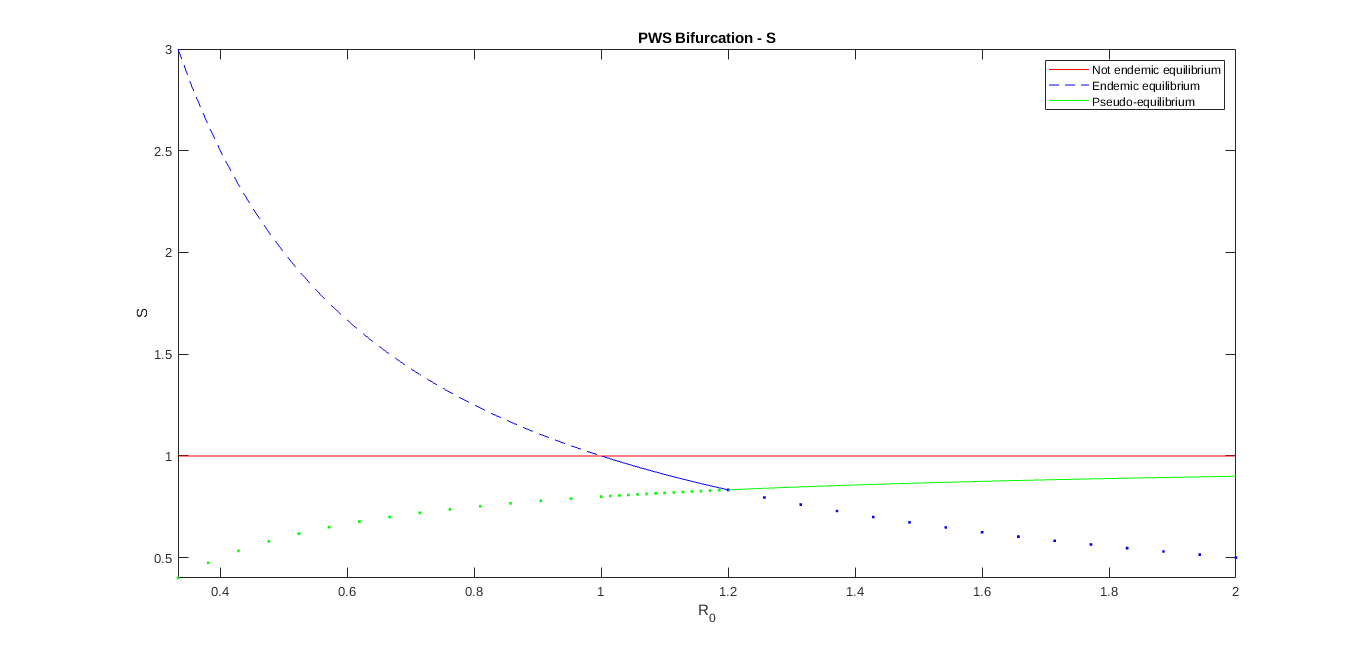
\includegraphics[width=\linewidth]{Figure/pws_bifurcation_s.png}  
        \caption{Bifurcation of S}
        \label{fig:pws_bifurcation_s}
    \end{subfigure}
    \begin{subfigure}{\textwidth}
        \centering
        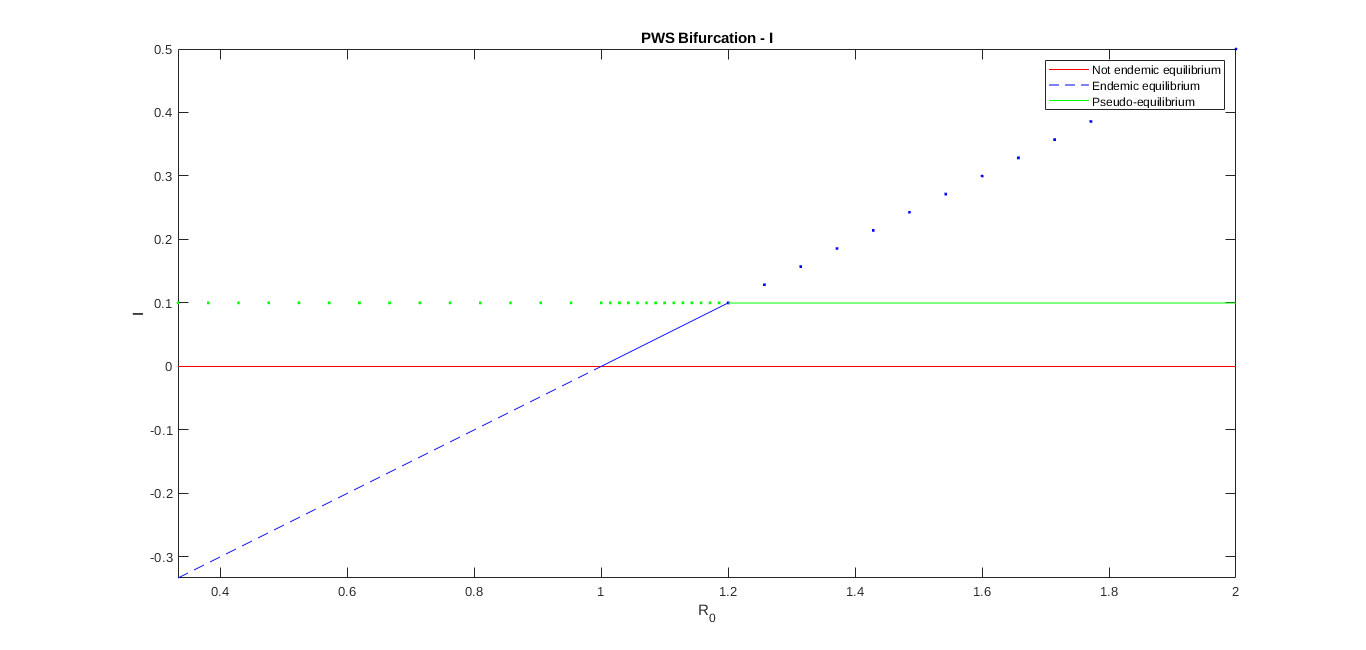
\includegraphics[width=\linewidth]{Figure/pws_bifurcation_i.png}  
        \caption{Bifurcation of I}
        \label{fig:pws_bifurcation_i}
    \end{subfigure}
    \caption{Bifurcation with parameters $\beta = 0.4$, $\mu = 0.2$, $\delta = 0.1$}
\end{figure}